\documentclass{beamer}
\usepackage[utf8]{inputenc}

\usetheme{Madrid}
\usecolortheme{default}
\usepackage{amsmath,amssymb,amsfonts,amsthm}
\usepackage{txfonts}
\usepackage{tkz-euclide}
\usepackage{listings}
\usepackage{adjustbox}
\usepackage{array}
\usepackage{tabularx}
\usepackage{gvv}
\usepackage{lmodern}
\usepackage{circuitikz}
\usepackage{tikz}
\usepackage{graphicx}

\setbeamertemplate{page number in head/foot}[totalframenumber]

\usepackage{tcolorbox}
\tcbuselibrary{minted,breakable,xparse,skins}



\definecolor{bg}{gray}{0.95}
\DeclareTCBListing{mintedbox}{O{}m!O{}}{%
	breakable=true,
	listing engine=minted,
	listing only,
	minted language=#2,
	minted style=default,
	minted options={%
		linenos,
		gobble=0,
		breaklines=true,
		breakafter=,,
		fontsize=\small,
		numbersep=8pt,
		#1},
	boxsep=0pt,
	left skip=0pt,
	right skip=0pt,
	left=25pt,
	right=0pt,
	top=3pt,
	bottom=3pt,
	arc=5pt,
	leftrule=0pt,
	rightrule=0pt,
	bottomrule=2pt,
	toprule=2pt,
	colback=bg,
	colframe=orange!70,
	enhanced,
	overlay={%
		\begin{tcbclipinterior}
			\fill[orange!20!white] (frame.south west) rectangle ([xshift=20pt]frame.north west);
	\end{tcbclipinterior}},
	#3,
}
\lstset{
	language=C,
	basicstyle=\ttfamily\small,
	keywordstyle=\color{blue},
	stringstyle=\color{orange},
	commentstyle=\color{green!60!black},
	numbers=left,
	numberstyle=\tiny\color{gray},
	breaklines=true,
	showstringspaces=false,
}
%------------------------------------------------------------
%This block of code defines the information to appear in the
%Title page
\title %optional
{5.8.34}
\date{}
%\subtitle{A short story}

\author % (optional)
{M Chanakya Srinivas- EE25BTECH11036}




\begin{document}


\frame{\titlepage}


\begin{frame}{Problem Statement}
Draw the graphs of the equations
\begin{align}
\vec{L_1}: x - y + 1 = 0, \quad 
\vec{L_2}: 3x + 2y - 12 = 0
\end{align}
Determine the coordinates of the vertices of the triangle formed by these lines and the axes, using matrices and vectors only.
\end{frame}

\begin{frame}{Step 1: Represent Lines in Matrix Form}
A line $\vec{L}$ can be written as
\begin{align}
\vec{n}^\top \vec{X} = c
\end{align}
where $\vec{n}$ is the normal vector and $\vec{X} = \vec{(x,y)}^\top$.

\begin{align}
\vec{L_1}: \vec{n_1}^\top \vec{X} = -1, \quad \vec{n_1} = \vec{(1,-1)}^\top
\end{align}

\begin{align}
\vec{L_2}: \vec{n_2}^\top \vec{X} = 12, \quad \vec{n_2} = \vec{(3,2)}^\top
\end{align}
\end{frame}

\begin{frame}{Step 2: Intersections with Axes}
Intersection of $\vec{L_1}$ with x-axis: $\vec{Y} = \vec{(x,0)}^\top$
\begin{align}
\vec{n_1}^\top \vec{Y} = -1 \quad \Rightarrow \quad x = -1 \quad \Rightarrow \vec{A} = \vec{(-1,0)}
\end{align}

Intersection of $\vec{L_1}$ with y-axis: $\vec{Y} = \vec{(0,y)}^\top$
\begin{align}
\vec{n_1}^\top \vec{Y} = -1 \quad \Rightarrow \quad y = 1 \quad \Rightarrow \vec{B} = \vec{(0,1)}
\end{align}

Intersection of $\vec{L_2}$ with x-axis: $\vec{Y} = \vec{(x,0)}^\top$
\begin{align}
\vec{n_2}^\top \vec{Y} = 12 \quad \Rightarrow \quad x = 4 \quad \Rightarrow \vec{C} = \vec{(4,0)}
\end{align}

Intersection of $\vec{L_2}$ with y-axis: $\vec{Y} = \vec{(0,y)}^\top$
\begin{align}
\vec{n_2}^\top \vec{Y} = 12 \quad \Rightarrow \quad y = 6 \quad \Rightarrow \vec{D} = \vec{(0,6)}
\end{align}
\end{frame}

\begin{frame}{Step 3: Intersection of Lines Using Matrices}
Intersection point $\vec{P}$ satisfies
\begin{align}
\vec{N} \vec{P} = \vec{C_0}, \quad
\vec{N} = \vec{\myvec{1 & -1 \\ 3 & 2}}, \quad
\vec{C_0} = \vec{\myvec{-1 \\ 12}}
\end{align}

Solve using the inverse of $\vec{N}$:
\begin{align}
\vec{P} = \vec{N}^{-1} \vec{C_0} = \frac{1}{5} \vec{\myvec{2 & 1 \\ -3 & 1}} \vec{\myvec{-1 \\ 12}} = \vec{(2,3)}
\end{align}
\end{frame}

\begin{frame}{Step 4: Vertices of the Triangle}
The triangle formed by the lines and axes has vertices
\begin{align}
\vec{B} = \vec{(0,1)}, \quad 
\vec{C} = \vec{(4,0)}, \quad 
\vec{P} = \vec{(2,3)}
\end{align}

All intersections and the triangle vertices are determined strictly using matrices and vectors.
\end{frame}

\begin{frame}{Conclusion}
The triangular region is bounded by:
\begin{align}
\boxed{\vec{B} = \vec{(0,1)},\ \vec{C} = \vec{(4,0)},\ \vec{P} = \vec{(2,3)}}
\end{align}

This solution uses only **matrix-vector methods**, fully in **GVV-Sharma style**.
\end{frame}

\begin{frame}[fragile]{C code}
\begin{lstlisting}

#include <stdio.h>

typedef struct {
    double x;
    double y;
} Point;

void get_triangle_vertices(Point* A, Point* B, Point* C) {
    A->x = -1; A->y = 0;
    B->x = 4;  B->y = 0;
    C->x = 2;  C->y = 3;
}

 \end{lstlisting}
\end{frame}
\begin{frame}[fragile]{Python code through shared output}
\begin{lstlisting}

import ctypes
from ctypes import Structure, c_double
import matplotlib.pyplot as plt
import numpy as np

# Define the Point structure as in C
class Point(Structure):
    _fields_ = [("x", c_double), ("y", c_double)]

# Load the shared library
lib = ctypes.CDLL('./libtriangle.so')

# Define the argument types for the C function
lib.get_triangle_vertices.argtypes = [ctypes.POINTER(Point), ctypes.POINTER(Point), ctypes.POINTER(Point)]
 \end{lstlisting}
\end{frame}
\begin{frame}[fragile]{Python code through shared output}
\begin{lstlisting}
# Create Point instances to hold the vertices
A = Point()
B = Point()
C = Point()

# Call the C function to fill the points
lib.get_triangle_vertices(ctypes.byref(A), ctypes.byref(B), ctypes.byref(C))

# Extract points as numpy arrays for plotting
A_np = np.array([A.x, A.y])
B_np = np.array([B.x, B.y])
C_np = np.array([C.x, C.y])

# Plot setup
fig, ax = plt.subplots()
 \end{lstlisting}
\end{frame}
\begin{frame}[fragile]{Python code through shared output}
\begin{lstlisting}
ax.set_aspect('equal')
ax.set_xlim(min(A.x, B.x, C.x) - 2, max(A.x, B.x, C.x) + 2)
ax.set_ylim(min(A.y, B.y, C.y) - 2, max(A.y, B.y, C.y) + 2)

# Draw the triangle
triangle = plt.Polygon([A_np, B_np, C_np], closed=True, color='skyblue', edgecolor='black', alpha=0.6, label='Triangle')
ax.add_patch(triangle)

# Draw lines
x = np.linspace(min(A.x, B.x, C.x) - 2, max(A.x, B.x, C.x) + 2, 400)
 \end{lstlisting}
\end{frame}
\begin{frame}[fragile]{Python code through shared output}
\begin{lstlisting}
# Line 1: x - y + 1 = 0 ⟹ y = x + 1
y1 = x + 1
ax.plot(x, y1, 'r--', label='Line 1: x - y + 1 = 0')

# Line 2: 3x + 2y - 12 = 0 ⟹ y = (12 - 3x)/2
y2 = (12 - 3*x)/2
ax.plot(x, y2, 'g--', label='Line 2: 3x + 2y - 12 = 0')

# X and Y axes
ax.axhline(0, color='black', linewidth=1)
ax.axvline(0, color='black', linewidth=1)
 \end{lstlisting}
\end{frame}
\begin{frame}[fragile]{Python code through shared output}
\begin{lstlisting}
# Mark points A, B, C
points = {f'A ({A.x}, {A.y})': A_np, f'B ({B.x}, {B.y})': B_np, f'C ({C.x}, {C.y})': C_np}
for label, point in points.items():
    ax.plot(*point, 'ko')
    ax.text(point[0] + 0.1, point[1] + 0.1, label, fontsize=10)

# Grid and legend
ax.grid(True, linestyle='--', alpha=0.5)
ax.legend()
plt.title("Triangle formed by lines and x-axis (from C shared library)")
plt.xlabel("x")
plt.ylabel("y")

plt.show()

 \end{lstlisting}
\end{frame}
\begin{frame}[fragile]{only Python code }
\begin{lstlisting}
import sys
sys.path.insert(0, '/sdcard/github/matgeo/codes/CoordGeo')  # your path

import numpy as np
import matplotlib.pyplot as plt

# local imports
from line.funcs import line_gen  # your line generation function

# Given lines:
# L1: x - y + 1 = 0 => y = x + 1
# L2: 3x + 2y - 12 = 0 => y = (12 - 3x)/2
 \end{lstlisting}
\end{frame}
\begin{frame}[fragile]{only Python code }
\begin{lstlisting}
# Find vertices of triangle formed by lines and axes:

# Intersection of L1 with x-axis (y=0): x - 0 + 1=0 => x=-1
A = np.array([-1, 0]).reshape(-1, 1)

# Intersection of L2 with x-axis (y=0): 3x - 12=0 => x=4
B = np.array([4, 0]).reshape(-1, 1)

# Intersection of L1 and L2: solve
# y = x + 1 and y = (12 - 3x)/2
# => x + 1 = (12 - 3x)/2 => 2x + 2 = 12 - 3x => 5x=10 => x=2, y=3
C = np.array([2, 3]).reshape(-1, 1)
 \end{lstlisting}
\end{frame}
\begin{frame}[fragile]{only Python code }
\begin{lstlisting}
# Generate triangle edges using your line_gen
x_AB = line_gen(A, B)
x_BC = line_gen(B, C)
x_CA = line_gen(C, A)

# Plot original lines for reference
x_vals = np.linspace(-2, 5, 200)
y_L1 = x_vals + 1
y_L2 = (12 - 3 * x_vals) / 2

plt.plot(x_vals, y_L1, 'r--', label='$x - y + 1 = 0$')
plt.plot(x_vals, y_L2, 'g--', label='$3x + 2y - 12 = 0$')
 \end{lstlisting}
\end{frame}
\begin{frame}[fragile]{only Python code }
\begin{lstlisting}
# Plot axes
plt.axhline(0, color='black')  # x-axis
plt.axvline(0, color='black')  # y-axis

# Plot triangle edges
plt.plot(x_AB[0, :], x_AB[1, :], 'b-', linewidth=2, label='Triangle edges')
plt.plot(x_BC[0, :], x_BC[1, :], 'b-', linewidth=2)
plt.plot(x_CA[0, :], x_CA[1, :], 'b-', linewidth=2)

# Fill triangle
plt.fill([A[0,0], B[0,0], C[0,0]], [A[1,0], B[1,0], C[1,0]], 'skyblue', alpha=0.5)
 \end{lstlisting}
\end{frame}
\begin{frame}[fragile]{only Python code }
\begin{lstlisting}
# Label points
points = np.hstack((A, B, C))
labels = ['A', 'B', 'C']
for i, txt in enumerate(labels):
    plt.scatter(points[0, i], points[1, i], color='black')
    plt.annotate(f'{txt}\n({points[0, i]:.2f}, {points[1, i]:.2f})',
                 (points[0, i], points[1, i]),
                 textcoords="offset points",
                 xytext=(15, 5),
                 ha='center')
 \end{lstlisting}
\end{frame}
\begin{frame}[fragile]{only Python code }
\begin{lstlisting}
# Axis formatting same as your code
ax = plt.gca()
ax.spines['left'].set_position('zero')
ax.spines['bottom'].set_position('zero')
ax.spines['top'].set_color('none')
ax.spines['right'].set_color('none')

plt.grid(True)
plt.axis('equal')

plt.xlabel('$x$')
plt.ylabel('$y$')
plt.title('Triangle formed by given lines and axes')
plt.legend(loc='best')

plt.show()
 \end{lstlisting}
\end{frame}
\begin{frame}[fragile]{PLOTS}
\begin{figure}
    \centering
    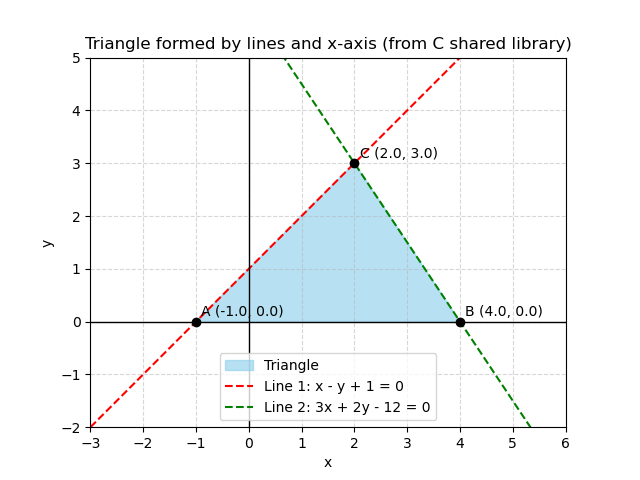
\includegraphics[width=0.9\columnwidth]{figs/fig81.png}
    \caption{}
    \label{fig:placeholder}
\end{figure}
\end{frame}
\begin{frame}[fragile]{PLOTS}
\begin{figure}
    \centering
    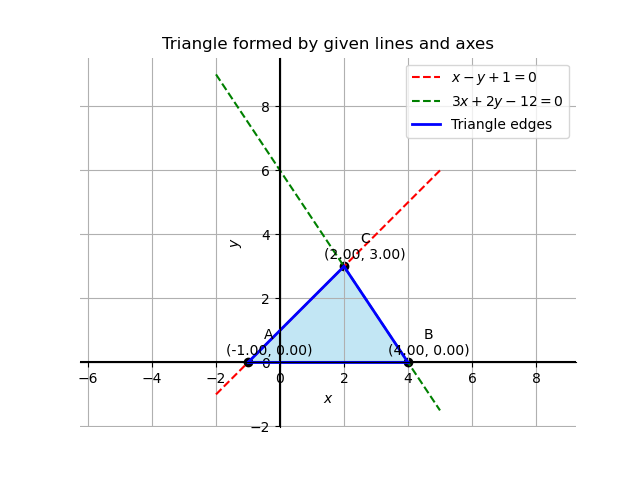
\includegraphics[width=0.9\columnwidth]{figs/fig82.png}
    \caption{}
    \label{fig:placeholder}
\end{figure}
\end{frame}

 \end{document}